\documentclass{pnastwo}
%\documentclass[10pt,twocolumn]{article}


%\usepackage[margin=1in]{geometry}
%\usepackage{graphicx}
\graphicspath{ {paper_figures2/} }

\usepackage{tikz}

\usepackage{float}
\usepackage{amssymb,amsfonts,amsmath}
\DeclareMathOperator*{\argmin}{arg\,min}

\makeatletter
\newcommand{\customlabel}[2]{%
\protected@write \@auxout {}{\string \newlabel {#1}{{#2}{}}}}
\makeatother

\renewcommand\thefigure{S\arabic{figure}}

\newcommand{\fig}[0]{Fig.}

\begin{document}



\begin{article}


\section{Materials and Methods}

\subsection{Image parameters}

The original image resolution is $1024 \times 1024$ pixels for the fixed images, and $512 \times 512$ pixels for the live images; all images are subsampled to $100 \times 100$ pixels for vector diffusion maps analysis.
%
A scale bar for a representative image is shown in \fig~\ref{fig:ap_dv}.
%
When imaging, the laser settings are calibrated so that images have good dynamic range, while not saturating the detector.
%
The same laser settings are maintained within each experiment.
%
The intensity of each channel is integer-valued, and ranges from $0$ (no signal) to $255$ (saturated). 
%
The Canny method is used to detect the edges of the nuclear signal in each image (using the \texttt{edge} function in MATLAB\textsuperscript{\textregistered}), and images are cropped to these edges to remove any size effects.
%
A constant $10$-pixel border is then added to each image. 
%
Contrast-limited adaptive histogram equalization (using the \texttt{adapthisteq} function with an $8 \times 8$ tile grid, and a uniform distribution for the intensities with a clip limit of 0.01) is used to normalize the intensities of the nuclear signal.
%
The nuclear signal is blurred using a disc filter with a $5$~pixel radius (using the \texttt{imfilter} function).
%
For the multichannel images, the nuclear signal is scaled by half (after normalization and blurring) relative to the other signals.


\subsection{Algorithms}

We will demonstrate the algorithms for registration and temporal ordering using a synthetic data set.
%
The relatively simple dynamics of this data set will allow us to easily visualize and illustrate the main features of the different algorithms.
%
Motivated by the geometry of our images, we construct a sequence of concentration profiles defined on a ring, and rotate each ring randomly around its center; an example is shown in \fig~\ref{subfig:1d_example}.
%
Rotation of the ring corresponds to shifting (with periodic boundary conditions) the one-dimensional concentration profile shown at the bottom of \fig~\ref{subfig:1d_example} (the symmetry group is $SO(2)$, the group of all two-dimensional proper rotations).
%
Each concentration profile is a noisy Gaussian (shown in \fig~\ref{subfig:1d_intensity}), and the Gaussians increase in intensity as a function of ``time".
%
We discretize the profiles into $100$ points, so our numerical data will be $100$-dimensional vectors (the corresponding symmetry group for the discretized profiles is $\mathbb{Z}_{100}$, the group of integers modulo $100$).
%
\fig~\ref{subfig:1d_unaligned_unordered} shows the entire data set; the concentration profiles have been stacked in an array, so that each row corresponds to a single profile.
%
Because the profiles are unregistered and unordered, the underlying dynamics (a Gaussian whose amplitude grows in time) are not readily apparent.



\subsubsection{Angular synchronization \cite{singer2011angular}}

Let $ x_1, \dots, x_m$ denote the signals that we wish to align with respect to rotations;
each signal is a function defined on the unit circle (on the plane).
%
%Practically, it is discretized in a $n$-long vector (the local intensity at $n$ equidistant points around the circle);
%rotating the function by an angle $\theta$ then corresponds to cyclically shifting the elements of $x_i$ by $\frac{\theta_i}{2 \pi} n$ (rounded to the nearest integer to obtain a valid shift).
%
First assume that each signal $x_i$ is a {\it noisy} rotated copy of the underlying signal $x_{true}$
(which we are {\it not} given), such that
\begin{equation}
x_i = f(x_{true}, \theta_i) + \xi_i
\end{equation}
where the function $f(x_{true}, \theta_i)$ rotates the signal $x_{true}$ by $\theta_i$ degrees, and $\xi_i$ is a (typically Gaussian) noise term.
%
Our goal is to recover $\theta_1, \dots, \theta_m$.
%
Up to noise,
\begin{equation} \label{eq:pairwise_rot}
x_i \approx f(x_j, \theta_i - \theta_j) ;
\end{equation}
note that \eqref{eq:pairwise_rot} does not require knowledge of $x_{true}$.
%
We can obtain an {\it estimate} of $\theta_i - \theta_j$ by computing the rotation that optimally aligns $x_j$ to $x_i$,
i.e., %$\theta_{ij} \approx \theta_i - \theta_j$, where
%
\begin{equation} \label{eq:opt_angle}
\theta_i - \theta_j \approx \theta_{ij} = \argmin_{\theta} \|x_i - f(x_j, \theta)\|^2.
\end{equation}
%
Practically, the signals are discretized in a $n$-long vector (the local intensity at $n$ equidistant points around the circle);
rotating the function by an angle $\theta$ then corresponds to cyclically shifting the elements of $x_i$
by $\frac{\theta_i}{2 \pi} n$ (rounded to the nearest integer to obtain a valid shift).
%
For the one-dimensional discretized profiles shown in \fig~\ref{fig:1d_demo}, we exhaustively search over all $n=100$ possible shifts of the signals to obtain the optimal angles in \eqref{eq:opt_angle}.
%
Alternatively, for continuous signals, an optimization algorithm
can be used \cite{ahuja2007template}.

Rather than work with the angles $\theta_{ij}$ directly, it is more convenient to consider the rotation matrices,
\begin{equation} \label{eq:R_theta}
R(\theta_{ij}) = \begin{bmatrix}
\cos(\theta_{ij}) & -\sin(\theta_{ij}) \\
\sin(\theta_{ij}) & \cos(\theta_{ij})
\end{bmatrix},
\end{equation}
which we can think of as operating on the points of the unit circle (on the plane) on which our signal is defined.
%
Successive rotations correspond to multiplication of the corresponding rotation matrices: $R(\alpha_1 + \alpha_2) = R(\alpha_1) R(\alpha_2)$.
%
Due to the orthogonality of rotation matrices, $R(-\alpha) = R(\alpha)^T$.

Let $d$ denote the dimension of the rotation matrices we are considering (for our example of planar rotations, $R(\theta_{ij}) \in \mathbb{R}^{2 \times 2}$ and $d=2$).
%
We construct the matrix $H \in \mathbb{R}^{md \times md}$, where $H$ is an $m \times m$ matrix of $d \times d$ blocks, with the $i,j^{th}$ block of $H$, $H_{ij}$, defined as
\begin{equation} \label{eq:H_to_R}
H_{ij} = R(\theta_{ij}).
\end{equation}
%
%
Under our assumption that $\theta_{ij} \approx \theta_i - \theta_j$, $H_{ij} \approx R(\theta_i) R(\theta_j)^T$
%\begin{equation}
%H_{ij} = R(\theta_{ij}) \approx R(\theta_i - \theta_j) = R(\theta_i) R(-\theta_j) = R(\theta_i) R(\theta_j)^T,
%\end{equation}
 and
\begin{equation} \label{eq:H_low_rank}
	H \approx
	\begin{bmatrix}
	R(\theta_1) \\
	R(\theta_2) \\
	\vdots \\
	R(\theta_m)
	\end{bmatrix}
	\begin{bmatrix}
	R(\theta_1)^T R(\theta_2)^T \dots R(\theta_m)^T
	\end{bmatrix}.
\end{equation}
%
It follows directly from \eqref{eq:H_low_rank} that the top block eigenvector of $H$ contains our best estimates of $R(\theta_1), R(\theta_2), \dots, R(\theta_m)$.
%
Let $\phi_1, \phi_2, \dots, \phi_{md}$ denote the eigenvectors of $H$ ordered so that $|\lambda_1| \ge |\lambda_2| \ge \dots \ge |\lambda_{md}|$, where $\lambda_i$ is the eigenvalue corresponding to $\phi_i$.
%
Then,
\begin{equation} \label{eq:R_hat}
\hat{R} =
\begin{bmatrix}
\hat{R}_1 \\
\hat{R}_2 \\
\vdots \\
\hat{R}_m
\end{bmatrix} =
\begin{bmatrix}
| & | & & | \\
\phi_1 & \phi_2 & \dots & \phi_d \\
| & | & & |
\end{bmatrix},
\end{equation}
where $\hat{R}_i \in \mathbb{R}^{d \times d}$ is (nearly) the estimate for $R(\theta_i)$.
%
To obtain our estimate of $R(\theta_i$), denoted $R_{i, est}$, we project $\hat{R}_i$ onto the closest orthogonal matrix,
\begin{equation} \label{eq:R_est}
R_{i, est} = U_i V_i^T,
\end{equation}
where $U_i$ and $V_i$ are the left and right singular vectors, respectively, of $\hat{R}_i$.
%
We adjust the sign of $\phi_1$ so that $det(R_{i, est}) = +1$, ensuring proper rotations 
(note that systematically incorporating improper rotations is also possible \cite{goemans1995improved, bandeira2013cheeger}).
%
We estimate $\theta_{i}$ by inverting \eqref{eq:R_theta}, and register the signals by rotating signal $i$ by $-\theta_i$.
%
We note that, in our actual computations, the pairwise rotations $\theta_{ij}$ are computed in a discrete setting, then the overall
synchronization is performed in the continuum context to obtain $\theta_i$, and the results are rounded to give the closest
discrete shift.

Importantly, this formulation also considers {\it higher-order} consistency information.
%
For example, given our pairwise estimates $R_{ij}$, we know that relationships of the form
\begin{equation} \label{eq:triplet_consistency}
R(\theta_{ik}) R(\theta_{kj}) \approx R(\theta_i) R(\theta_k)^T R(\theta_k) R(\theta_j)^T = R(\theta_i) R(\theta_j)^T
\end{equation}
should also hold.
%
Note that
\begin{equation}
(H^2)_{ij} = \sum_k R(\theta_{ik}) R(\theta_{kj});
\end{equation}
therefore, {\it all} information of the form in \eqref{eq:triplet_consistency} is contained in the matrix $H^2$ (and higher order
consistency information in its higher powers).
%
Because $H$ and $H^2$ have the same eigenvectors, our problem formulation accounts for not only pairwise alignment information, but also these higher-order considerations.

\subsubsection{Diffusion maps \cite{coifman2005geometric}}

Given $m$ data points $x_1, \dots, x_m$ (typically vectors in a high-dimensional vector space), we want to find a coordinate transformation $y(x)$ that preserves local geometry: points that are ``close" in the original space should also be ``close" in the coordinates $y$.
%
The first step is to construct the matrix $W \in \mathbb{R}^{m \times m}$, where $W_{ij}$ is large if points $x_i$ and $x_j$ are ``close.''
%
We use a diffusion kernel,
\begin{equation} \label{eq:dmaps_W}
W_{ij} = \exp \left( -\frac{d^2(x_i, x_j)}{\epsilon^2} \right),
%W_{ij} = e^{ -\frac{d^2(x_i, x_j)}{\epsilon^2}}
\end{equation}
where $d(x_i, x_j)$ is a pairwise distance between $x_i$ and $x_j$ (often the Euclidean distance), and $\epsilon$ is a characteristic scale.
%
Points less than $\epsilon$ apart are thus considered ``close'' and points farther than $\epsilon$ apart are considered ``far away''.
%
$\epsilon$ can be chosen using several techniques (see, for example \cite{coifman2008graph, rohrdanz2011determination}); here, we take $\epsilon^2$ to be $1/10^{th}$ of the median of the squared pairwise distances.

To find the coordinate $y$, we want solve the following optimization problem \cite{Belkin2003}
\begin{equation} \label{eq:dmaps_opt_problem}
\argmin_{y} \sum_{ij} W_{ij} (y(x_i) - y(x_j))^2.
\end{equation}
%
We first compute the diagonal matrix $D$, where $D_{ii} = \sum_{j=1}^{m} W_{ij}$, and the matrix $A$, where
\begin{equation} \label{eq:dmaps_A}
A = D^{-1} W.
\end{equation}
%
We calculate the eigenvectors $\phi_1, \phi_2, \dots, \phi_m$, ordered such that $|\lambda_1| \ge |\lambda_2| \ge \dots \ge |\lambda_m|$.
%
Because the matrix $A$ is similar to the symmetric matrix $D^{-1/2} W D^{-1/2}$, $A$ is guaranteed to have real eigenvalues and real, orthogonal eigenvectors.
%
Because the matrix $A$ is row-stochastic, $\lambda_1=1$ and $\phi_1$ is a constant vector; this is a trivial solution to \eqref{eq:dmaps_opt_problem}.
%
%In general, the next few eigenvectors $\phi_2, \dots, \phi_m$ give ``meaningful'' embedding coordinates for the data, such that $\phi_j(i)$ gives the $j^{th}$ embedding coordinate of the $i^{th}$ data point.
%
The next eigenvector, $\phi_2$, is the (non-trivial) solution to \eqref{eq:dmaps_opt_problem}, so that $\phi_2(j)$, the $j^{th}$ entry of $\phi_2$, gives the ``new" coordinate for data point $x_j$ (i.e., $\phi_2(j) = y(x_j)$).
%
In our application, we have assumed that this {\em single} direction of variability, parameterized by $\phi_2$, is one-to-one with time.
%
Ordering the data by $\phi_2(j)$ will then, effectively, order them in time.
%
The procedure generalizes when the data lie on higher-dimensional manifolds (not just curves) in data space, where leading eigenvectors can give subsequent embedding coordinates for the data.
%

\subsubsection{Vector diffusion maps\cite{singer2012vector}}

In vector diffusion maps, given data points $x_1, \dots, x_m$, one first constructs the matrix $S \in \mathbb{R}^{md \times md}$, with the $i,j^{th}$ block of $S$, $S_{ij}$, defined as
\begin{equation} \label{eq:vdm_S}
	S_{ij} = A_{ij} H_{ij}
\end{equation}
%
where $A_{ij} \in \mathbb{R}$ (defined in \eqref{eq:dmaps_A}) pertains to the diffusion kernel between data points, and $H_{ij} \in \mathbb{R}^{d \times d}$ (defined in \eqref{eq:H_to_R}) pertains to the pairwise alignment between data points.
%
It is important to note that distance $d(x_i, x_j)$ used in the diffusion kernel in \eqref{eq:dmaps_W} is the distance between data points {\it after} after pairwise alignment, i.e., the minimum distance between all possible shifts of the two data points (which is obtained in \eqref{eq:opt_pairwise}).
%
In the language of symmetry groups, this distance is a metric between the orbits induced by the relevant symmetry group.

One then computes the eigenvalues $\lambda_1, \lambda_2, \dots, \lambda_{md}$ and eigenvectors $\phi_1, \phi_2, \dots, \phi_{md}$ of $S$, ordered such that $|\lambda_1| \ge |\lambda_2| \ge \dots \ge |\lambda_{md}|$.
%
These eigenvectors contain information about {\it both} the optimal rotations (the ``synchronization" component) and the
variation of the data {\it after} the spatial symmetries have been factored out (in our case, their temporal variation).
%
Assuming that the data (after symmetries have been factored out) are relatively closely clustered, it is reasonable
to expect, as in angular synchronization, that the top (block) eigenvector of $S$ contains approximations of the optimal rotations,
which can be computed in the same way from \eqref{eq:R_est}.
%
We then expect subsequent eigenvectors to contain information about the main direction(s) of data variability modulo the geometric symmetries.
%%%
%%% somewhere we need to talk about compact groups
%%% discussion might be a good place because SCALING is obviously important and
%%% it is not compact......
%%%
%However, the eigenvectors now also contain information about the embedding coordinates for our images.
%

In general, the embedding coordinates are given by
\begin{equation} \label{eq:vdm_coord}
\psi_{k,l} (i) = \langle \phi_k(i), \phi_l(i) \rangle,
\end{equation}
where $\phi_k(i) \in \mathbb{R}^d$ denotes the $i^{th}$ block of $\phi_k$,
%
If we assume that the rotations and the dynamics are uncoupled and therefore separable, then the eigenvectors of $S$ have the following structure: each block eigenvector contains estimates of the optimal rotations (up to a constant rotation) multiplied by the corresponding embedding coordinate (a scalar)
%
As the first diffusion maps coordinate is constant over the data, the first block eigenvector contains only the optimal rotations.
%
The second block eigenvector (eigenvectors $d+1$ through $2d$) contains the optimal rotations, each multiplied by their second diffusion maps coordinate.
%
We can therefore recover this diffusion maps coordinate by taking inner products of the columns of the second block eigenvector with columns of the first block eigenvector.
%%
%%YGK just as a favor to me, tell me how consistent the three values are -- 
%%
The $j^{th}$ embedding coordinate will be given by $\psi_{k,l}$, where $jd +1 < k \le (j+1)d$ and $1 \le l \le d$,
and we select $k, l$ such that the coordinate $\psi_{k, l}$ has the largest variability, i.e., the $j^{th}$ coordinate is $\psi_{k,l}$, where $k, l$ is the solution to
\begin{equation} \label{eq:first_embed_vdm}
\max_{
\begin{matrix}
jd +1 \le k \le (j+1)d \\
1 \le l \le d
\end{matrix}}
 \sum_i \psi_{k,l} (i)^2. 
\end{equation}

\begin{table}[t]
%\caption{Outline of algorithm used to temporally order images}
\setlength{\fboxrule}{2pt}
\framebox[\columnwidth]{
\begin{minipage}{0.9\columnwidth}
{\bf Outline of algorithm used to register and order images}
\begin{enumerate}
\item Compute the alignments for each pair of images, as described in \eqref{eq:opt_pairwise}.
Retain both the optimal pairwise rotations as well as the minimum distances obtained when pairs are optimally aligned.
%
\item Compute the corresponding rotation matrices $R(\theta_{ij})$ from \eqref{eq:R_theta}.
%
\item Select $\epsilon$ for use in the diffusion maps kernel. 
%
Taking $\epsilon$ to be on the order of the median of the pairwise distances often yields good results. 
\item Compute the matrix $S$ in \eqref{eq:vdm_S}. 
$A_{ij}$ is computed from \eqref{eq:dmaps_W} and \eqref{eq:dmaps_A}, using the pairwise distances from step 1, and $H_{ij} = R(\theta_{ij})$ are computed in step 2.
%
\item Compute the eigenvalues  $\lambda_1, \lambda_2, \dots, \lambda_{3m}$ and eigenvectors $\phi_1, \phi_2, \dots, \phi_{3m}$ of $S$, ordered such that $|\lambda_1| \ge |\lambda_2| \ge \dots \ge |\lambda_{3m}|$.
%
\item Estimate the optimal three-dimensional rotation for each image: stack the first three eigenvectors $\phi_1, \phi_2, \phi_3$ into a $3m \times 3$ matrix, and then divide this matrix into $m$ $3 \times 3$ blocks, $\hat{R}_1, \dots, \hat{R}_m$. Compute the estimated rotations for each of these $m$ blocks as in \eqref{eq:R_est}. If most of the rotations are improper ($det(R) = -1$), flip the sign of one of the eigenvectors.
\item Multiply each estimated rotation $R_{i, est}$ by $R_{1, est}^T$ (so that $R_{1, est}$ will become the identity matrix).
\item For each image $i$, compute the optimal rotation to align the image by converting $R_{i, est}^T$ (note the transpose) to the corresponding angle using \eqref{eq:R_theta}. 
\item Compute the first embedding coordinate $\psi_{k,1}(i)$ as described in \eqref{eq:vdm_coord} and \eqref{eq:first_embed_vdm}, where $3 \le k \le 4$.
\item To order the images, sort them by the values of this embedding coordinate $\psi_{k,1}(i)$.
\end{enumerate} 
\end{minipage}
}
\end{table}


\subsection{Registering images} \label{subsec:trans_rot_register}

To register sets of images, 
the first step is to compute the optimal alignments between pairs of images.
%
Practically, we have square images discretized as pixels (rather than continuous functions on the plane).
%
For each image pair $I_i$ and $I_j$ we compute
\begin{equation}\label{eq:opt_pairwise}
\theta_{ij} = \argmin_{
0^\circ \le \theta < 360^\circ }
 \|g(I_j, \theta) - I_i \|^2.
\end{equation}
where $g(I_j, \theta)$ is image $I_j$ rotated around the center of the square by $\theta$ degrees.
%
The norm, $\| \cdot \|$, is the Euclidean norm between the pixel intensities of the channels.
%
The domain of the image (a square) is not invariant to our rotations; however, the pixels near the corners of the square have zero intensity, and so the norm can be meaningfully computed as long as the main image does not ``move out of'' the original square.
%
Image rotation is performed with the \texttt{imwarp} function in Matlab, using linear interpolation to estimate the pixel intensities after rotation.
%
The missing pixels in the corners of the rotated image are taken to have zero intensity.
%
The solution to \eqref{eq:opt_pairwise} is not easily computed, as the objective function will most likely be nonconvex.
%
Therefore, instead of using an optimization procedure, we discretize the search space and exhaustively search to find the solution (for the results presened, we use $10^\circ$ discretization steps).
%
%We discritize the search space of rotations into 20 possible rotations %($d\theta  \in \{0, \pi/10, \pi/5, \dots, 9 \pi/5, 19\pi/10 \}$),
%and 11 possible translations in both . %($dx, dy \in \{-20, -16, -12, \dots, 12, 16, 20 \}$).
%
%We check all possible combinations for the rotation and translations that best align $I_j$ to $I_i$.
%
Although computationally demanding, this ``embarrassingly parallelizable" direct enumeration approach is not prohibitive here.
%
Once we have computed $\theta_{ij}$ for all image pairs, we can proceed with the vector diffusion maps procedure.
%
The rotation matrices returned from vector diffusion maps can be used to calculate the angle of rotation for each image (by inverting \eqref{eq:R_theta}), and the function $g$ as described previously is then used to rotate the images.

\subsection{The eigenvalue spectrum}

We can use the distribution of the eigenvalues from (vector) diffusion maps to help deduce the dimensionality of the data.
%
In diffusion maps, the largest eigenvalue will always be 1 and correspond to the trivial (constant) eigenvector, and $|\lambda_k|$ gives a measure of the importance of coordinate $\phi_k$. 
%
Therefore, we expect to see a ``spectral gap'' in the eigenvalues which separates the meaningful coordinates from those corresponding to noise.
%
However, some embedding coordinates which appear meaningful according to the eigenvalues may be harmonics of previous coordinates \cite{ferguson2010systematic}.
%
Therefore, one must visually check for correlations among potential embedding coordinates before deducing the true dimensionality of the data. 

In vector diffusion maps, the importance of each coordinate is measured by the product of the corresponding eigenvalues (i.e., the importance of $\psi_{k,l}$ is given by $| \lambda_k \lambda_l |$). 
%
We again expect to see a ``spectral gap'' in these eigenvalue products between those corresponding to meaningful coordinates (modulo higher harmonics) and those corresponding to noise. 


\subsection{Smooth trajectories from registered and ordered images}

Once we have registered and ordered the images, we can smooth the resulting trajectory to obtain a ``stereotypic" developmental trajectory.
%
Let $I_1, \dots, I_m$ denote the set of {\em registered and ordered} images (so $I_j$ is the $j^{th}$ image in the ordered set).
%
We define the average image at time $\tau$, denoted $\overline{I}_{\tau}$ (where $1 \le \tau \le m$), as a (Gaussian) weighted average of the images,
\begin{equation}
\overline{I}_{\tau} =  \frac{\sum_j \exp \left( - \frac{|j - \tau|^2}{\sigma^2} \right) I_i}{\sum_j \exp \left( - \frac{|j - \tau|^2}{\sigma^2} \right) }
\end{equation}
where $\sigma$ is the scale of the Gaussian filter.
%
For the images in \fig~4, we take $\sigma = 3$.
%
See \cite{kemelmacher2011exploring} for a more detailed discussion.


\bibliographystyle{pnas2}
\bibliography{../image_analysis_paper/background_reading/references,../../references/references}


\end{article}

\begin{figure}
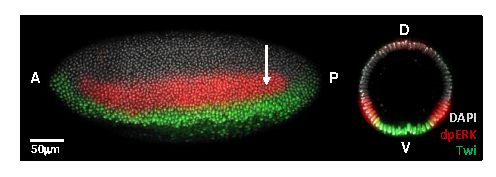
\includegraphics{figS1}
\caption{(Left) A lateral view of a {\it Drosophila} embryo stained with DAPI (gray), dpERK (red), and Dorsal (green). The embryo is presented so that the anterior (A) side is to the left and the posterior (P) side is to the right. The arrow indicates the position(s) where the cross-section of an embryo is imaged. (Right) A dorsoventral view of the cross-section of the {\it Drosophila} embryo. The dorsal (D) side is up and the ventral (V) side is down. Images were collected at the focal plane $\sim 18\%$ from the posterior pole of an embryo (right arrow in the left image). }
\label{fig:ap_dv}
\end{figure}

\begin{figure}
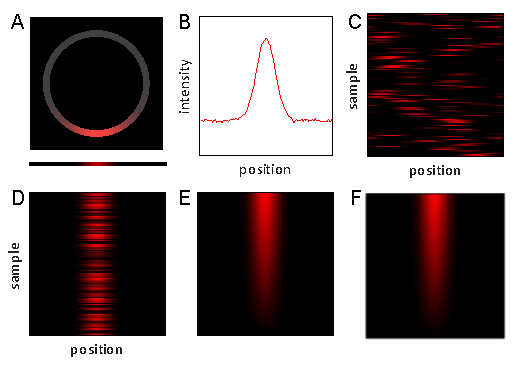
\includegraphics{figS2}
\caption{Synthetic data set used to illustrate the data processing algorithms. {\it (A)} One-dimensional concentration profile on a ring (top), and the corresponding profile on a line (bottom). {\it (B)} Intensity corresponding to the profile in {\it A}. {\it (C)} An ensemble of concentration profiles, each of the form described in {\it A}. Each row in the array corresponds to a single profile. {\it (D)} The profiles in {\it C}, now registered using angular synchronization. {\it (E)} The profiles in {\it D}, now temporally ordered using diffusion maps. {\it (F)} The profiles in {\it C}, registered and temporally ordered in a single step using vector diffusion maps.}
\label{fig:1d_demo}
%\customlabel{fig:1d_demo}{3}
\customlabel{subfig:1d_example}{\ref{fig:1d_demo}{\it A}}
\customlabel{subfig:1d_intensity}{\ref{fig:1d_demo}{\it B}}
\customlabel{subfig:1d_unaligned_unordered}{\ref{fig:1d_demo}{\it C}}
\customlabel{subfig:1d_aligned_unordered}{\ref{fig:1d_demo}{\it D}}
\customlabel{subfig:1d_aligned_ordered}{\ref{fig:1d_demo}{\it E}}
\customlabel{subfig:1d_aligned_ordered_vdm}{\ref{fig:1d_demo}{\it F}}
\end{figure}

\begin{figure*}
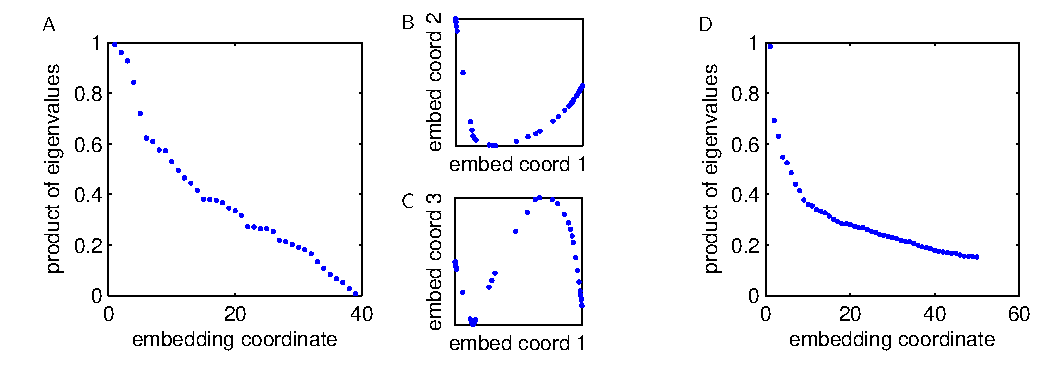
\includegraphics{figS3}
\caption{Eigenvalue spectra. {\it (A)} Eigenvalue spectrum for the live imaging data set presented in \fig~3. Note that there is a gap after the third coordinate. {\it (B), (C)} Second and third embedding coordinates, respectively, versus the first embedding coordinate for the live imaging data set presented in \fig~3. Note that coordinates 2 and 3 are harmonics/functions of coordinate 1, and are therefore not informative about structure in the data set.  We can conclude that the data set is effectively one-dimensional. {\it (D)} Eigenvalue spectrum for the live imaging data set presented in \fig~4. Note that there is a gap after the first coordinate; we can conclude that the data set is effectively one-dimensional. }
\end{figure*}

\begin{figure*}
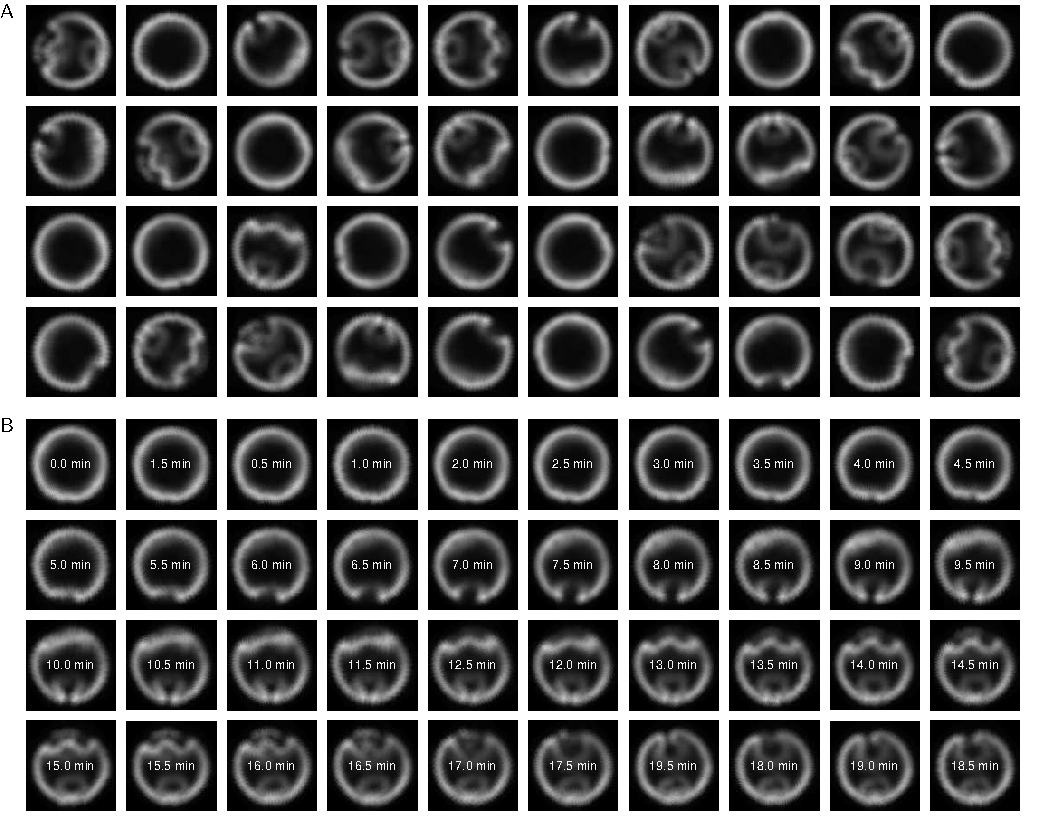
\includegraphics{figS4}
\caption{Live imaging data set. {\it (A)} Live imaging data set used for the results in \fig~3. The images have been preprocessed as described above, each image has been arbitrarily rotated, and the order of the images has been shuffled. {\it (B)} Data set from A after registration and ordering. The real time for each image is indicated. }
\end{figure*}

\begin{figure*}
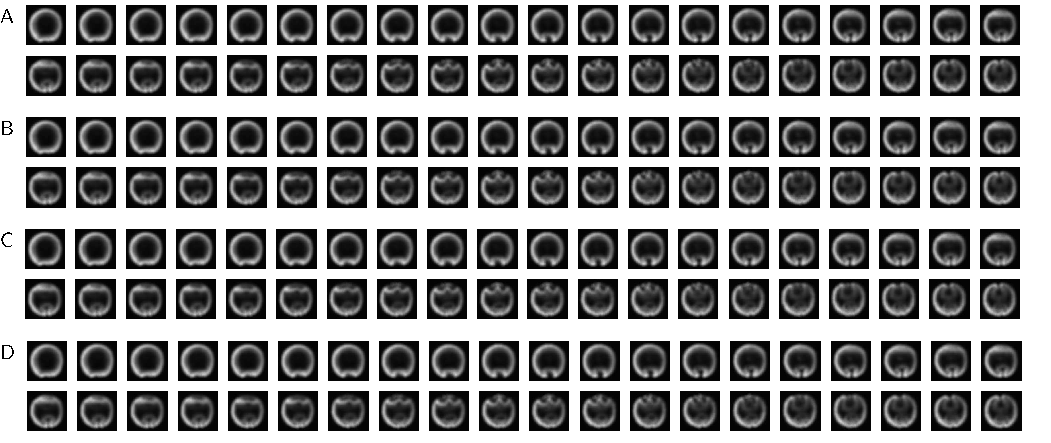
\includegraphics{figS5}
\caption{{\it (A-D)} Four additional live imaging data sets used for the analysis in \fig~3. }
\end{figure*}

\begin{figure*}	
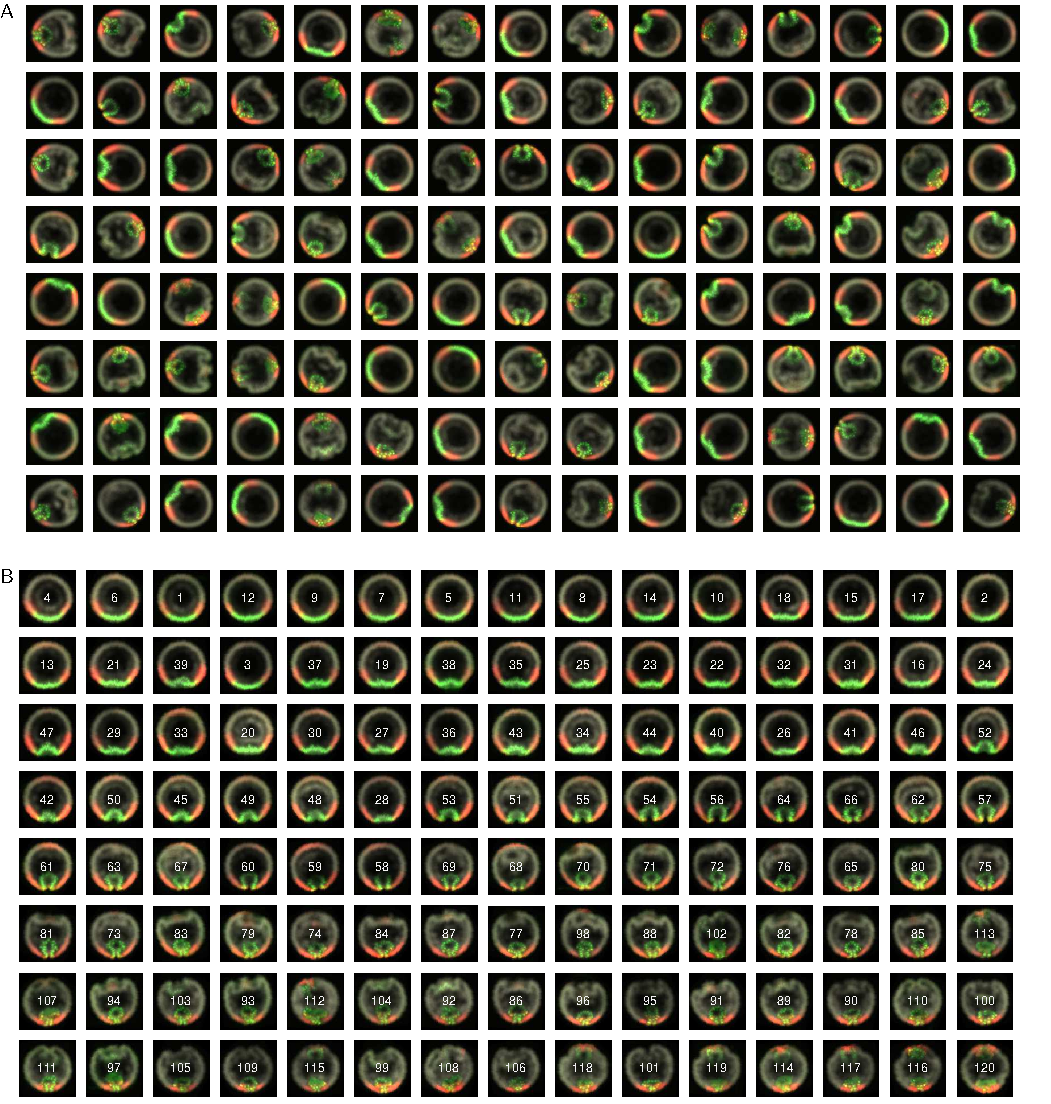
\includegraphics{figS6}
\caption{Fixed embryo imaging data set. {\it (A)} Fixed images used for the results in \fig~4. The images have been preprocessed as described above. {\it (B)} Data set from A after registration and ordering. The expert rank for each image is indicated. }
\end{figure*}



\end{document} 